\documentclass[]{scrartcl}
\usepackage[utf8]{inputenc} 
\usepackage[T1]{fontenc}
\usepackage[upright]{fourier} 
\usepackage[usenames,dvipsnames]{xcolor}
\usepackage{tkz-kiviat,numprint,fullpage} 
\usepackage{pgfplots}
\pgfplotsset{compat=1.16}


\usetikzlibrary{arrows}
\thispagestyle{empty}
\begin{document} 
	
	
	
	
	\begin{figure}[htbp!]
		\centering
		\begin{tikzpicture}
			\tkzKiviatDiagram[scale=.75,label distance=.5cm,
			radial  = 5,
			gap     = 1,  
			lattice = 7]{Typ 1,Typ 2,Typ 3,Typ 4 ,Typ 5, Typ 6}
			%Jonathan
			\tkzKiviatLine[thick,color=blue,mark=none!20,opacity=.85](6,4,3,2,1,2)
			%Annabell
			\tkzKiviatLine[thick,color=green,mark=none!20,opacity=.85](6,5,7,2,2,3)
			%Luise
			\tkzKiviatLine[thick,color=yellow,mark=none!20,opacity=.5](6,4,6,2,2,3)
			%(T) Ben-Luca
			\tkzKiviatLine[thick,color=lime,mark=none!20,opacity=.85](5,3,3,1,0,1)
			%Benny
			\tkzKiviatLine[thick,color=magenta,mark=none!20,opacity=.85](6,5,7,2,0,3)
			%Mohammed
			\tkzKiviatLine[thick,color=orange,mark=none!20,opacity=.85](6,5,7,2,1,3)
			%Yufei
			\tkzKiviatLine[thick,color=brown,mark=none!20,opacity=.85](6,2,7,0,1,1)
			%Henrik
			\tkzKiviatLine[thick,color=purple,mark=none!20,opacity=.85](0,2,3,1,1,3)
			%Namenslos
			\tkzKiviatLine[thick,color=teal,mark=none!20,opacity=.85](6,5,7,2,2,3)
			%Maximalwert
			\tkzKiviatLine[thick,color=black,mark=none,
			fill=black!20,opacity=1](6,5,7,2,2,3)
			\tkzKiviatGrad[prefix=,unity=1](1)  
		\end{tikzpicture}
		\caption[Auswertung]{Auswertung der Tests}
		\label{auswertung}
	\end{figure}
	
	% Please add the following required packages to your document preamble:
	

	\begin{table}[htpb!]
		\begin{tabular}{|l|l|l|l|l|l|l|l|}
			\hline
			Name         & Typ 1 & Typ 2 & Typ 3 & Typ 4 & Typ 5 & Typ 6 & Total \\ \hline
			Jonathan     & 6     & 4     & 3     & 2     & 1     & 2     & 17    \\ \hline
			Annabell     & 6     & 5     & 7     & 2     & 2     & 3     & 25    \\ \hline
			Luise        & 6     & 4     & 6     & 2     & 2     & 3     & 23    \\ \hline
			(T) Ben-Luca & 5     & 3     & 3     & 1     & 0     & 1     & 13    \\ \hline
			Benny        & 6     & 5     & 7     & 2     & 0     & 3     & 23    \\ \hline
			Mohammed     & 6     & 5     & 7     & 2     & 1     & 3     & 24    \\ \hline
			Yufei        & 6     & 2     & 7     & 0     & 1     & 1     & 17    \\ \hline
			Henrik       & 0     & 2     & 3     & 1     & 1     & 3     & 10    \\ \hline
			Namenlos     & 6     & 5     & 7     & 2     & 2     & 3     & 25    \\ \hline
			Maximalwert  & 6     & 5     & 7     & 2     & 2     & 3     & 25    \\ \hline
		\end{tabular}
		\caption{Erreichte Punkte pro Kategorie}
		\label{tab:data}
	\end{table}

\begin{figure}[htbp!]
	\centering
	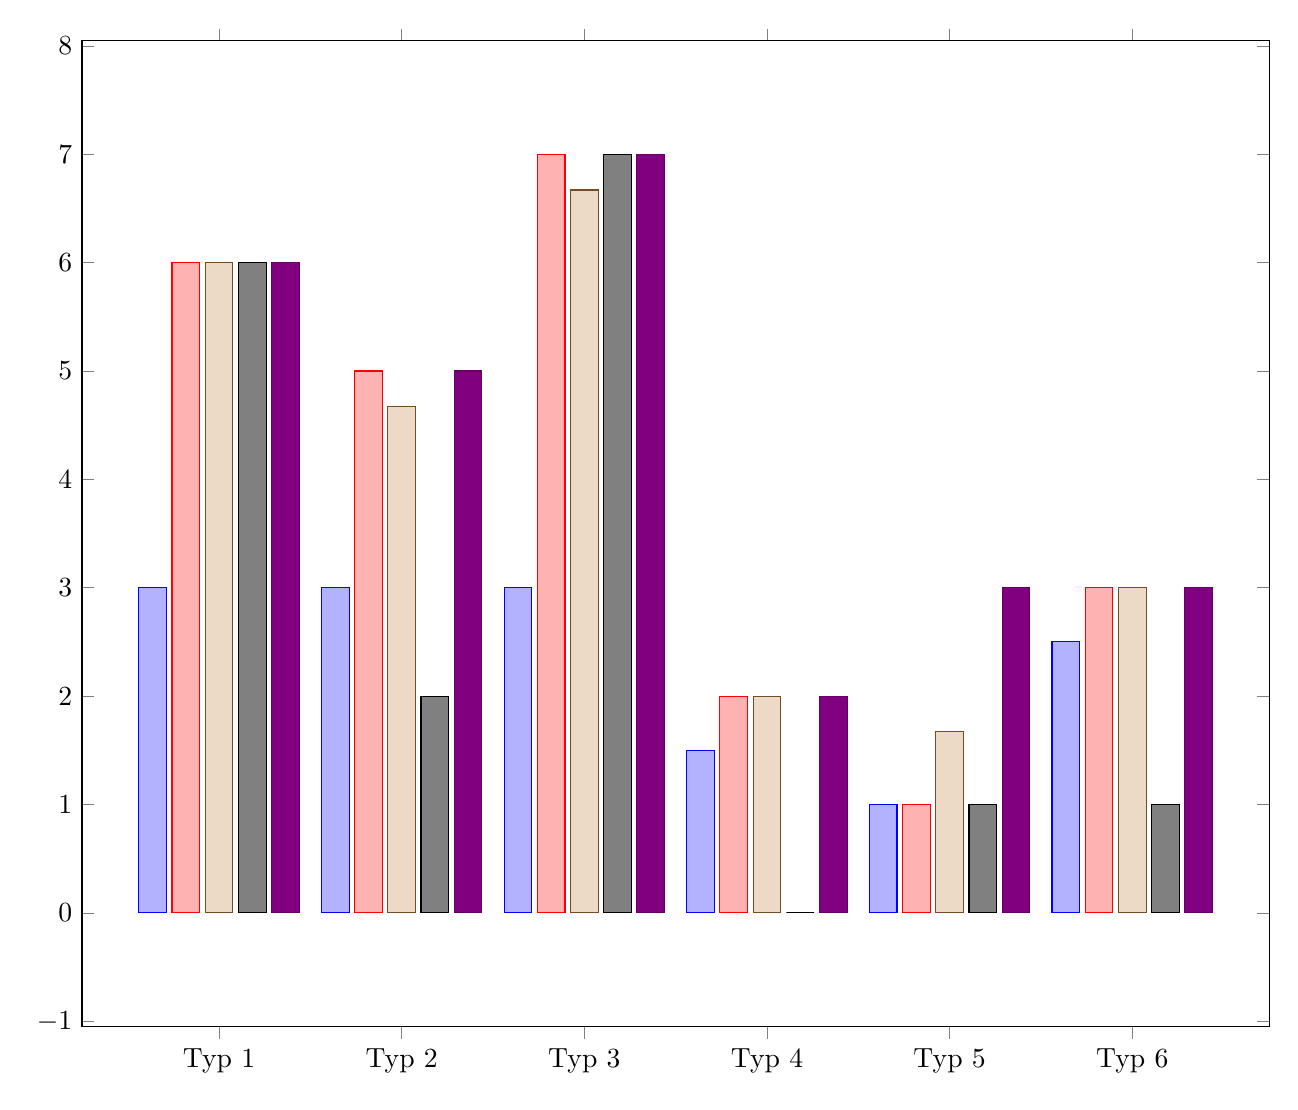
\begin{tikzpicture}
		\begin{axis}[
			ybar,enlargelimits=0.15,
			symbolic x coords={Typ 1, Typ 2, Typ 3, Typ 4, Typ 5, Typ 6},xtick={Typ 1, Typ 2, Typ 3, Typ 4, Typ 5, Typ 6 
			}, scale = 2.2
			]
			%Border Collie
			\addplot coordinates
			{(Typ 1,3) (Typ 2,3) (Typ 3,3) (Typ 4,1.5) (Typ 5,1) (Typ 6,2.5)};
			%Erdmännchen
			\addplot coordinates
			{(Typ 1,6) (Typ 2,5) (Typ 3,7) (Typ 4,2) (Typ 5,1) (Typ 6,3)};
			%Elefant
			\addplot coordinates
			{(Typ 1,6) (Typ 2,4.67) (Typ 3,6.67) (Typ 4,2) (Typ 5,1.67) (Typ 6,3)};
			%Panda
			\addplot coordinates
			{(Typ 1,6) (Typ 2,2) (Typ 3,7) (Typ 4,0.0) (Typ 5,1) (Typ 6,1)};
			%Maximum
			\addplot coordinates
			{(Typ 1,6) (Typ 2,5) (Typ 3,7) (Typ 4,2) (Typ 5,3) (Typ 6,3)};
		\end{axis}
	\end{tikzpicture}
	\caption[Auswertung Durchschnitt]{Durchschn. Punkte pro Kategorie der einzelnen Typen (Border Collie, Erdmännchen, Elefant, Panda, Maximum)}
	\label{auswertung_typus}
\end{figure}

	
	
\end{document}